\section{Experiments}
In this section, we will describe the implementation of our mathematical formula detection system and dataset in detail.
\subsection{Dataset}
Our data is from the \href{https://zenodo.org/record/4757865}{IBEM dataset}. This originally comprises $600$ documents, with $8273$ pages in total. Those documents are parsed from mathematical papers, then each page is annotated with a bounding box of 2 types: isolated and embedded. The dataset is then split into various sets for ICDAR 2021 Competition on Mathematical Formula Detection, including Training, Test, and Validation sets. \\
\textbf{Training}
\begin{itemize}
\item Tr00: $4082$ pages.
\item Tr01: $760$ pages.
\item Tr10: $329$ pages.
\end{itemize}
\textbf{Validation}
\begin{itemize}
\item Va00: $577$ pages.
\item Va01: $380$ pages.
\end{itemize}
\textbf{Test}
\begin{itemize}
\item Ts00: $736$ pages.
\item Ts01: $380$ pages.
\item Ts10: $699$ pages.
\item Ts11: $329$ pages.
\end{itemize}
Our experiment uses Tr01, Tr10, Ts01 for training, Va01 for validation, and Ts11 for testing with $2178$ pages in total ($ \sim 26.33\% $ of the original dataset), and an approximate ratio of $4.47:1.16:1.$ The reason for this small subset is for the purpose of evaluating the ability of the model on small subsets, and the performance it gives (F1-score) through time (minutes).\\
The numbers of embedded and isolated bounding boxes in each set are:
\begin{itemize}
\item \textbf{Training:} $31074$ embedded bounding boxes, $6617$ bounding boxes.
\item \textbf{Validation:} $6595$ embedded bounding boxes, $1346$ bounding boxes.
\item \textbf{Test}: $5702$ embedded bounding boxes, $1074$ bounding boxes.
\end{itemize}
\begin{figure}[H]
\centering{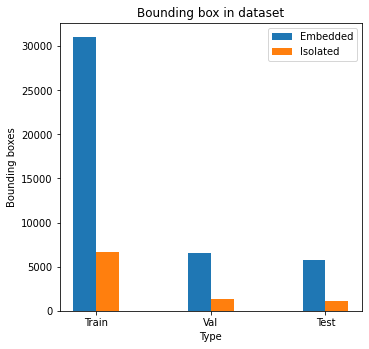
\includegraphics[scale=0.5]{dataset/bounding_box}}
\caption{The numbers of embedded and isolated bounding boxes}
\end{figure}

\subsection{Implementation Details}
Our baseline model is Faster R-CNN with ResNet50 as the backbone. We have trained on Kaggle with a 4-core CPU, 12GB RAM, and a NVIDIA Tesla P100 GPU \footnote{\url{https://www.kaggle.com/docs/notebooks}}. The images are resized to $1447 \times 2048$ with the same ratio. The size of the region crops from the image is $1200 \times 1120$ to fit the limitation of the machine. They are also flipped and padded for data augmentation. For the feature aggregation, we use FPN (2-6). The loss function for the classifier is Cross-Entropy Loss and for the bouding box is L1 Loss. Test images are resized to $1583 \times 2048$ due to the distribution of the test dataset, flip augmentation is also applied. For post-processing, Non-Maximum Suppression (NMS) with $0.5$ IoU threshold to remove redundant boxes. All models are trained based on the MMDetection toolbox and config given by \href{https://github.com/Yuxiang1995/ICDAR2021_MFD/blob/main/configs/_base_/models/faster_rcnn_r50_fpn.py}{Yuxiang Zhong}. The optimizer for this baseline is Stochastic Gradient Descent (SGD) with a learning rate of $0.02.$  
\subsection{Remarks}
We have tested on 3 configs: Faster R-CNN with schedule 1x ($12$ epochs), \href{https://github.com/hkzhang95/DynamicRCNN}{Dynamic R-CNN} with schedule 1x ($12$ epochs) to check if it is better than the faster one and Faster R-CNN with schedule 2x ($24$ epochs) to check if the model is underfitting with low epochs.\\
The results are given in the figures below. 
%\newpage
\begin{figure}[H]
\centering{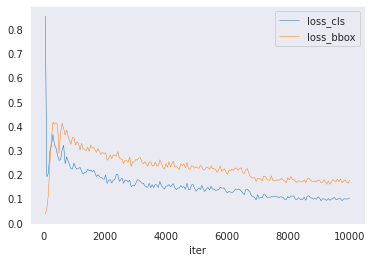
\includegraphics[scale=0.7]{loss/v2_1x}}
\caption{Faster R-CNN with schedule 1x}
\end{figure}

\begin{figure}[H]
\centering{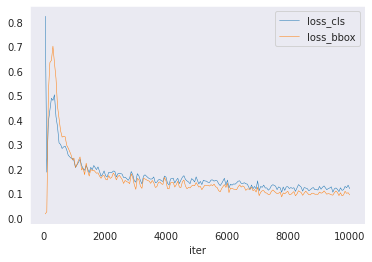
\includegraphics[scale=0.7]{loss/v5_1x}}
\caption{Dynamic R-CNN with schedule 1x}
\end{figure}

\begin{figure}[H]
\centering{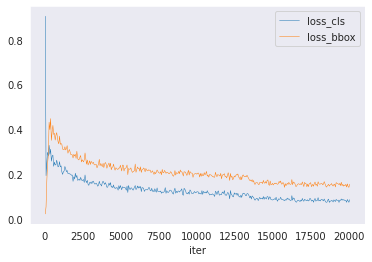
\includegraphics[scale=0.7]{loss/v2_2x}}
\caption{Faster R-CNN with schedule 2x}
\end{figure}

The F1-score gained from the model is as follow.
\begin{figure}[H]
\centering{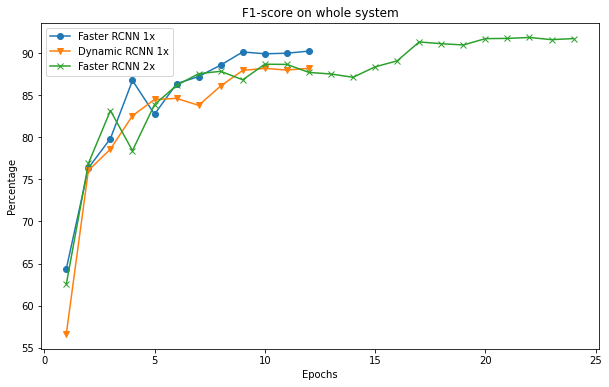
\includegraphics[scale=0.4]{f1-score/whole}}
\caption{F1-score on whole system}
\end{figure}

\begin{figure}[H]
\centering{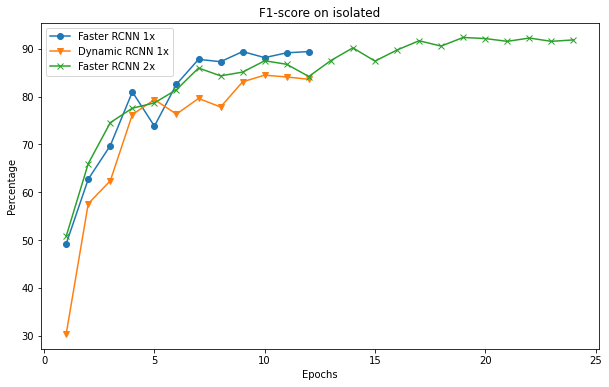
\includegraphics[scale=0.4]{f1-score/isolated}}
\caption{F1-score with isolated bounding box}
\end{figure}

\begin{figure}[H]
\centering{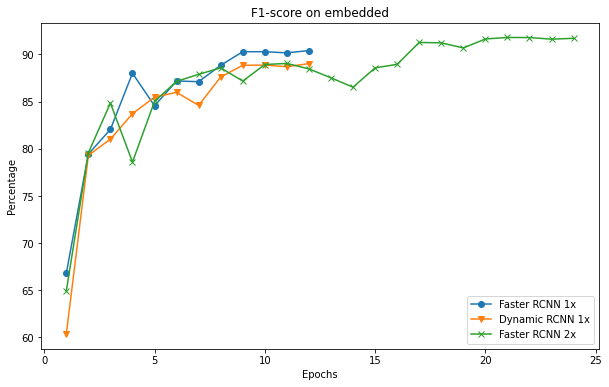
\includegraphics[scale=0.4]{f1-score/embedded}}
\caption{F1-score with embedded bounding box}
\end{figure}
%\newpage
It can be seen from the graphs that on the whole system, with the same schedule 1x, the F1-scores given by the Faster R-CNN model are higher than the one by Dynamic R-CNN if we use the same number of epochs, except in the case of $5$ epochs. The difference gets higher when we increase the number of epochs. Compared to the scores by Faster R-CNN with schedule 2x ($24$ epochs), although it gives a lower percentage when trained with a small number of epochs, the score becomes increasing to around $90\%$. Moreover, on the isolated bounding box, the Faster R-CNN model shows its benefit when compared with the number of Dynamic R-CNN, the F1-score of Faster R-CNN is nearly 90$\%$ while the one of Dynamic R-CNN reaches about 80$\%$ when they are both trained with $12$ epochs. Considering the Faster R-CNN with schedule 2x, it gives the same F1-score with Dynamic R-CNN 1x at the point of $12$ epochs, however,  the score is about $90\%$ at the point of $24$ epochs.  Besides that, it can be inferred from the figures of the embedded bounding box that with the same number of epochs ($12$ epochs), the Faster R-CNN model always provides better results than the Dynamic R-CNN, in spite of the fact that the difference is not large. When we increase the number of epochs to $24,$ we can observe that the F1-score of Faster R-CNN can reach the milestone of nearly $95\%.$\\
From the result given above, we can conclude that the Faster R-CNN model gives better F1-score than the Dynamic R-CNN model.

